\documentclass[11pt, a4paper, oneside, portrait]{article}
\usepackage[utf8]{inputenc}
\usepackage[T2A, T1]{fontenc}
\usepackage[british, french, russian]{babel}
\usepackage[style=ieee]{biblatex}
\usepackage[most]{tcolorbox}
\usepackage{graphicx}
% \usepackage{animate}
\usepackage{xurl}
\usepackage{setspace}
\usepackage{ragged2e}
\usepackage{indentfirst}
\usepackage{mathptmx}
\usepackage{pdfpages}
\usepackage{geometry}
\usepackage{amsmath}
\usepackage{amssymb}
\usepackage{txfonts}
\usepackage{multicol}
\usepackage{fancyhdr}
\usepackage{wrapfig}
\usepackage{array}
\usepackage{float}
\usepackage{alltt}
\usepackage{tabularx}
\usepackage{caption}
\usepackage{fancyvrb}
\usepackage{fvextra}
\usepackage{enumitem}
\usepackage{bigfoot}
\usepackage{hyperref}
\geometry{
    a4paper,
    top=2cm,
    bottom=2cm,
    right=2cm,
    left=2cm
}
\hypersetup{
    colorlinks = true,
    linkcolor = blue,
    urlcolor = blue,
    filecolor = blue,
    citecolor = blue
}
\pagestyle{fancy}
\fancyhf[HC]{\textbf{MU4RBI01 --~Projet \emph{Python}}}\fancyhf[HL]{\thepage}\fancyhf[HR]{\thepage}
\fancyhf[FC]{\thepage}

\author{E{\small{}LION} G{\small{}ALIBA} Fady, N{\small{}OCHÉ} Kévin \&{} S{\small{}IVATHASAN} Ramya}
\title{\textbf{MU4RBI01 --~Projet \emph{Python}}}
\date{\today}


\begin{document}
    \selectlanguage{french}\justifying
    \maketitle

    \section*{Introduction}
        Ce présent document a pour but d'expliquer comment le projet python de l'UE \emph{MU4RBI01} de \emph{Sorbonne Université}, département scientifique, a été travaillé par le groupe n°5 de la formation d'IPS-TSDM (auteur de ce rapport).

        Le projet a été réalisé grâce à \emph{Github}, via l'intermédiaire de \emph{Git}.
        Les logiciels tels que \emph{Kate} ou \emph{Konsole} ont été essentiels au bon déroulement du projet. % IMPORTANT: Rajouter vos applications!

        Le repository du projet peut être retrouvé via cet URL: \url{https://github.com/NKevinVI/Sorbonne\_SdI\_IPS\_TSDM\_MU4RBI01\_Project}

    \section*{Fonctionnalités du jeu}
        %

%     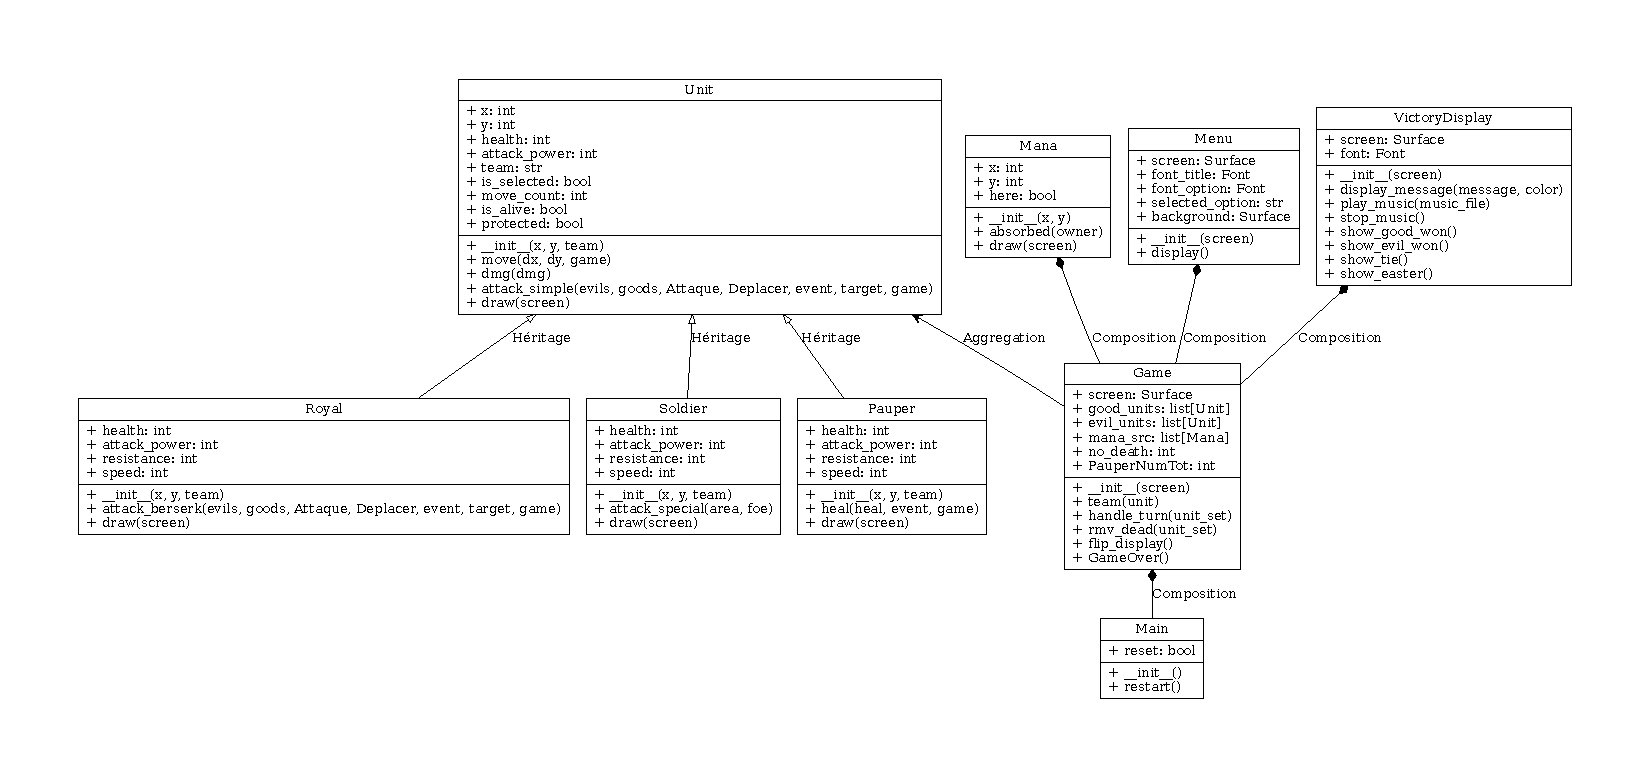
\includepdf[noautoscale=true]{UML.pdf} % À décommenter une fois le diagramme UML créé.
\end{document}
